% Auto-generated by scripts/02c_build_ea18_family_composition_inflation_annex.R.
\section{Inflation by Household Composition}
\label{sec:app-family-composition-inflation}

This appendix extends Figure~\ref{fig:ea-household-group-inflation} by grouping households according to family composition. The five categories are mutually exclusive: single adults; couples without children; single parents with one or more children; couples with one child; and couples with two or more children.

\begin{figure}[H]
\centering
\caption{Year-on-year inflation by household composition, 18-country HBS sample}
\label{fig:app-family-composition-inflation}
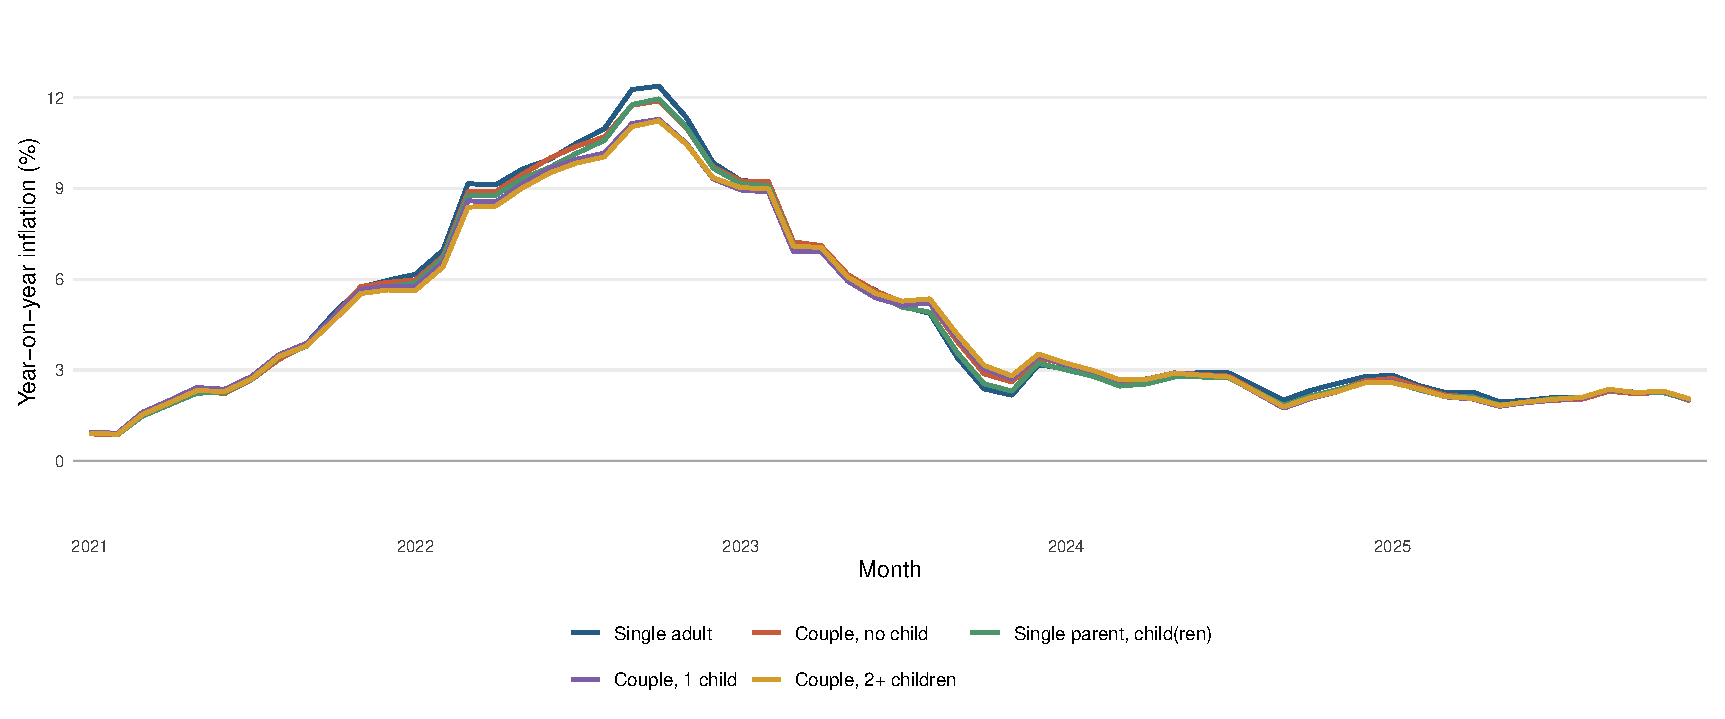
\includegraphics[width=0.99\textwidth]{fig/fig_EA18_2021_2025_inflation_family_composition_annex.pdf}
\vspace{6pt}
\captionsetup{font=footnotesize, format=hang, singlelinecheck=false, justification=justified}
\caption*{Notes: Household-specific annual inflation rates are calculated from 2020 HBS expenditure baskets and monthly HICP prices at COICOP digit 3, using the same RAS and country-aggregation procedure as Figure~\ref{fig:ea-household-group-inflation}. Family types are identified from MB05: a couple contains the reference person and a spouse or partner, and a child is a member recorded as the child of either adult. Households that also contain parents, other relatives, non-relatives, or unspecified members are excluded. Sources: Eurostat HBS 2020 scientific-use files and HICP; authors' calculations.}
\end{figure}
